
Consider the paradifferential formulation of the wave maps problem. To apply the gauge covariant estimates, one needs to show that terms with high-high interactions are indeed perturbative. For the small data problem, this follows immediately from the multi-linear and energy estimates. Define the \emph{energy dispersion norm} by
	\[ ||\phi||_{\sfED[I]}= \sup_{k \in \Z} ||P_k \phi||_{L^\infty_{t, x} [I]}. \]

\begin{theorem}[Energy-dispersed regularity theorem]
	There exist functions $F(\cE) \gg 1$ and $\epsilon (\cE) \ll 1$ of energy such that if $\phi : [t_0, t_1] \times \R^2 \to \MM$ is a solution to the wave maps equation \eqref{wave} with finite energy $\cE[\phi] \equiv \cE$ and energy dispersion
		\begin{equation}
			||\phi||_{\sfED [I]} \leq \epsilon (\cE), 
		\label{eq:ED}
		\end{equation}
	then 
		\begin{equation}
			||\phi||_{\sfS [I]} \leq \cF(\cE).
		\label{eq:S}
		\end{equation}
	In addition, there exists a polynomial $K(\cF)$ such that if $\{c_\kappa\}_\kappa$ is any $(\delta_0, \delta_1)$-admissible frequency envelope for $\vec \phi_0$, we have the bound 
		\[ ||\phi||_{\sfS_c [I]} \leq K(\cF(E)).  \]
	In particular, one may extend $\phi$ to a finite energy wave-map on the interval $(t_0 - T, t_1 + T)$ for some $T \ll_{\cE, c, \epsilon} 1$. \label{thm:ED}
\end{theorem}

\subsection{Induction on energy}

To illustrate the induction on energy scheme, we will aim for a qualitative statement, though as we detail the proof we will arrive at the full quantitative energy-dispersion theorem. We say that an energy $\cE$ is \emph{regular} if there exists parameters $\epsilon \ll 1$ sufficiently small and $\cF \gg 1$ sufficiently large such that for every wave map $\phi : I \times \R^2 \to \MM$ with energy $\cE [\phi] = \cE$ we have
	\[ ||\phi||_{\sfED [I]} \leq \epsilon \text{ implies } || \phi||_{\cS[I]} \leq \cF. \]
We remark that we are free to choose these parameters $\epsilon$ and $\cF$, though as we will soon see in the proof we can give a quantitative dependence on $\cE[\phi]$. Let us denote the set of regular energies by 
	\[ \cR := \{ \cE \in [0, \infty) : \text{$\cE$ is a regular energy} \}. \]
The global well-posedness theorem for small energy furnishes the base case for our induction on energy, $[0, \cE_0] \subseteq \cR$ for $\cE_0 \ll 1$ sufficiently small. Assume then for induction that energies are regular up to some $\cE_0$. Our goal is to construct a positive non-increasing function of energy $e (\cE) > 0$ to push the induction forward by showing that $\cE_0 + e$ is a regular energy for any $e \leq e (\cE_0)$. This induction step allows us to conclude the usual continuous induction argument, as it shows
	\begin{itemize}
		\item $\cR$ is open: if $[0, \cE_0] \subseteq \cR$ then $[0, \cE_0 + e(\cE_0)] \subseteq \cR$, 
		\item $\cR$ is closed: if we have a sequence of regular energies $\{ \cE_n \}_n \subseteq \cR$ such that $\cE_n \nearrow \cE$, then since $e :[0, \infty) \to (0, \infty)$ is positive non-increasing, $e(\cE_n) > e(\cE) > 0$. Taking $n$ large, we have $\cE \leq \cE_n + e(\cE_n)$ and therefore by the induction step $\cE$ is regular. 
	\end{itemize}
By connectedness, we conclude $\cR = [0, \infty)$, i.e. all energies are regular. 

\begin{remark}
	If instead $e(\cE_n) \to 0$ as $\cE_n \nearrow \cE$, e.g. if we were not precise and allowed $e$ to depend also on $\epsilon$ or $\cF$, then we would not be able to prove closedness of the set of regular energies. The Kenig-Merle strategy is to assume towards a contradiction that there exists a \emph{critical element}, i.e. a minimal energy blow-up solution, and then attempt to eliminate this possibility. 
	
	\begin{figure}[h]
		\begin{center}
			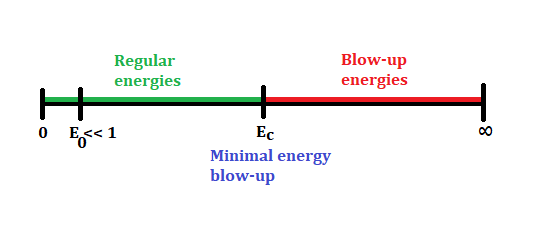
\includegraphics{graphics/kenigmerle}
			\caption{If the set of regular energies $\cR$ was not closed, i.e. $\cR = [0, \cE_c)$, then there would exist a minimal energy blow-up wave map $\cE [\phi_c] = \cE_c$. }
		\end{center}
	\end{figure}
\end{remark}

We end this subsection by getting the proof of the induction step started. Suppose for induction $\cE_0$ is a regular energy and $e \leq e(\cE_0) \ll 1$ a small energy increment to be chosen later. Let $\phi : I \times \R^2 \to \MM$ be a wave map with energy $\cE[\phi] = \cE_0 + e$ and energy dispersion 
	\[ ||\phi||_{\sfED[I]} \leq \epsilon.\]
We want to compare with a wave map $\widetilde \phi : I \times \R^2 \to \MM$ with an energy by hypothesis assumed to be regular $\cE[\widetilde \phi] = \cE_0$. Choose then a \emph{cut frequency} $k_* \in \R$ to truncate the initial data  such that its projection $\Pi$ back onto $T\mathbb M$ has regular energy,
	\[ \cE[\Pi P_{\leq k_*}  \phi[0]] = \cE_0. \]
Such a projection is well-defined since energy-dispersed solutions stay close to the manifold. Local well-posedness guarantees that there exists a solution $\widetilde \phi : J \times \R^2 \to \MM$ with initial data $\widetilde \phi[0] = \Pi P_{\leq k_*}  \phi[0]$ on some small time interval $J \subseteq I$. To make use of the fact $\cE_0$ is a regular energy, we need to pass the energy dispersion of $\phi$ to $\widetilde \phi$. The heuristic is that $\widetilde \phi[0] \approx P_{\leq k_*} \phi[0]$ up to higher-order errors. Indeed, 
	\begin{equation}
		||P_k (P_{\leq k_*} \phi [0] - \widetilde \phi[0]) ||_{\dot H^1 \times L^2} \lesssim_{\cE_0} \epsilon^{\frac14} 2^{-\frac12 |k - k_*|}. \label{eq:seedzero}
	\end{equation}
The proof uses standard Moser-type estimates, i.e. chain rule and Bernstein's inequality, see \cite[Section 11]{SterbenzTataru2010}. The gain on the right-hand side allows us to use the Sobolev-Bernstein inequality to estimate the energy-dispersion of $\widetilde \phi$ at time $t = 0$ by 
	\begin{align*}
		||P_k \widetilde \phi [0]||_{L^\infty_x}
			&\leq ||P_k (P_{\leq k_*} \phi [0] - \widetilde \phi[0]) ||_{L^\infty_x} + ||P_k (P_{\leq k_*} \phi [0]||_{L^\infty_x} \\
			&\lesssim_{\cE_0} 2^{\frac{k}{2}} ||P_k (P_{\leq k_*} \phi [0] - \widetilde \phi[0]) ||_{\dot H^1 \times L^2}  + ||P_k \phi[0]||_{L^\infty_x}\lesssim_{k^*} \epsilon^{\frac14} + \epsilon \lesssim \epsilon^{\frac14}. 
	\end{align*}
Choosing then $\epsilon^{\frac14} \ll \epsilon (\cE_0)$, the local well-posedness theory guarantees that $\widetilde \phi$ is energy-dispersed in that, after possibly choosing a smaller time interval $J_0 \subseteq J \subseteq I$,  
	\[ ||\widetilde\phi||_{\sfED[J_0]} \leq \epsilon (\cE_0).  \]
Then the induction hypothesis guarantees that we have the dispersive bound
	\[ ||\widetilde \phi ||_{\sfS [J_0]} \leq \cF (\cE_0).  \]


\subsection{Bootstrap argument}

We want to propagate $\sfS$-control for the evolution of low frequencies $\widetilde\phi$ to our original solution $\phi$. We also want to propagate our estimates from the sub-interval $J \subseteq I$ to the full time interval $I$. To this end, suppose we have suitable choices of $e, \epsilon, \cF$, and let $\phi$ be a wave map such that 
	\begin{equation}
		||\phi||_{\sfED [I]} \leq \epsilon.
		\label{eq:ED1}
	\end{equation}
We make the following bootstrap assumptions on the sub-interval $J \subseteq I$,
	\begin{align}
		||\phi||_{\sfS [J]}
			&\leq 2 \cF , \label{eq:BS1}\\
		||\widetilde \phi||_{\sfED [J]}
			&\leq \widetilde \epsilon \label{eq:BS2}.
	\end{align}
The second bootstrap assumption along with the induction on energy hypothesis imply
	\begin{align}
		||\widetilde \phi||_{\sfS [J]} 
			\leq \widetilde \cF.
		\label{eq:induction}
	\end{align}	
We aim to improve the bootstrap assumptions to 
	\begin{align}
		||\phi||_{\sfS [J]}
			&\leq \cF, \label{eq:BS1i} \\
		||\widetilde \phi||_{\sfED [J]}
			&\leq \frac12\widetilde\epsilon \label{eq:BS2i}. 		
	\end{align}		
To conclude the proof of Theorem \ref{thm:ED}, we need some technical but nonetheless easy results which allow us to use the usual bootstrap argument.  First, we need to check that the improved bounds \eqref{BS1i} and \eqref{BS2i} on some base case interval $J_0$. This is done by propagating our good energy bounds at time $t = 0$.

\begin{lemma}[Seed bound]
	Let $\phi : I \times \R^2 \to \mathbb M$ be an affinely Schwartz function and $\{c_k\}_k$ a frequency envelope. If $I_n \subseteq I$ is a decreasing sequence of intervals converging to $t = 0$, then 
		\begin{align}
			\lim_{n \to \infty} ||\phi||_{\sfS[I_n]}
					&\lesssim ||\phi[0]||_{\dot H^1 \times L^2},  \\
				\lim_{n \to \infty} ||\phi||_{\sfS_c [I_n]}
					&\lesssim ||\phi[0]||_{(\dot H^1 \times L^2)_c}. 	
			\end{align}		
\end{lemma}

\begin{proof}
	Follows from the energy estimate. 
\end{proof}

Next, we show that the norms in question depend continuously on the endpoints of the intervals. This allows us to use the improved bounds \eqref{BS1i} and \eqref{BS2i} to push the continuous induction forward. 

\begin{lemma}[Continuity properties]
	Let $\phi : I \times \R^2 \to \mathbb M$ be an affinely Schwartz function and $\{c_k\}_k$ a frequency envelope. For each sub-interval $J \subseteq I$, we have that $\phi \in \sfS[J] \cap \sfS_c [J]$, and its $\sfS$-norm $||\phi||_{\sfS[J]}$, its $\sfS_c$-norm $||\phi||_{\sfS_c[J]}$, and its energy-dispersion norm $||\phi||_{\sfED[J]}$ all depend continuously on the endpoints of $J$. 
\end{lemma}

\begin{proof}
	For the $\sfS$-norm, use scale invariance and the fact that convergence in the Schwartz topology is stronger that convergence in $\sfS$-norm. For the frequency envelope modification $\sfS_c$, the proof for each dyadic piece uses the same argument as before, while smallness of the tail frequencies allows us to conclude. A similar argument holds for the $\sfED$-norm. 
\end{proof}

Finally, we show that the bootstrap assumptions \eqref{BS1} and \eqref{BS2} form a closed condition, and good estimates allow us to extend the wave map, so the improvement really is an open condition. 

\begin{lemma}[Closure and extension property]
	Let $\phi : I \times \R^2 \to \mathbb M$ be a classical wave map and $\{c_k\}_k$ a frequency envelope. If $I_n$ is an increasing sequence of intervals such that $\bigcup_n I_n = I$ and 
			\begin{align*}
				||\phi||_{\sfS[I_n]} 
					&\leq \cF, \\
				||\phi||_{\sfED [I_n]} 
					&\leq \epsilon,
			\end{align*}		
		then $\phi \in \sfS[I]$. Furthermore, it can be extended to a classical wave map in a larger interval. 
\end{lemma}

\begin{proof}
	Use the frequency envelope local well-posedness result. 
\end{proof}



\subsection{Comparing $\phi$ and $\widetilde\phi$}

It remains to improve our bootstrap assumptions \eqref{BS1}, \eqref{BS2} to the estimates \eqref{BS1i}, \eqref{BS2i}. We divide the analysis between comparing low frequencies and comparing high frequencies. 

\subsubsection{Low frequencies}

We use the \textit{a priori} space-time control \eqref{BS1} for our solution $\phi$ to pass good energy dispersion estimates \eqref{ED1} for $\phi$ back down to the truncated solution $\widetilde\phi$, improving \eqref{BS2} to \eqref{BS2i}. Towards this end it suffices to compare $\widetilde \phi$ against the frequencies of $\phi$ below the cut frequency $k_*$. We claim that there exists a non-decreasing positive function $K_1 (\cF) > 0$ of polynomial growth such that 
	\[
		|| \widetilde \phi - P_{\leq k_*} \phi||_{\sfS[J]} \leq K_{1} (\cF) \epsilon^{\delta_0}.
	\]
Given this estimate, choosing $\epsilon \ll \widetilde\epsilon \ll 1$ such that $K_{1} (\cF) \epsilon^{\delta_0} \ll \widetilde \epsilon$, it follows that
	\[
		||\widetilde \phi ||_{\sfED [J]}
			\lesssim || \widetilde \phi - P_{\leq k_*} \phi||_{\sfS[J]} + ||\phi ||_{\sfED[J]} \leq K_{1} (\cF) \epsilon^{\delta_0} + \epsilon \leq \frac12 \widetilde\epsilon,
	\]
improving our energy dispersion bound \eqref{BS2} to \eqref{BS2i}, as desired.

The difference $\psi := \widetilde \phi - \phi_{\leq k_*}$ satisfies the equation 
	\[
		\Box \psi = - \bfS(\widetilde \phi) \partial^\alpha \widetilde \phi \partial_\alpha \widetilde\phi + P_{\leq k_*}(\bfS(\phi) \partial^\alpha \phi \partial_\alpha \phi).
	\]

\begin{proposition}[Low frequency evolution]\label{prop:lowfreq}
	Let $\phi$ be a wave map with energy $\cE[\phi] = \cE + e$, and denote $\widetilde \phi$ the wave map with initial data $\widetilde \phi[0] = \Pi P_{\leq k_*} \phi[0]$ and energy $\cE[\widetilde \phi] = \cE$. If $\phi$ and $\widetilde \phi$ are defined on the time interval $J$ with bounds
		\begin{align}
			||\phi||_{\sfED[J]} 
				&\leq \epsilon, \\
			||\phi||_{\sfS[J]}
				&\leq \cF, 	
		\end{align}
	and
		\begin{align}
			||\widetilde\phi||_{\sfED[J]} 
				&\leq \widetilde\epsilon, \\
			||\widetilde\phi||_{\sfS[J]}
				&\leq \widetilde\cF, 	
		\end{align}	
	for appropriate choices of $\epsilon, \widetilde\epsilon, \cF, \widetilde\cF$, then there exists a non-decreasing positive function $K_{1}(\cF) > 0$ of polynomial growth such that 
	\begin{equation}
		|| \widetilde \phi - P_{\leq k_*} \phi||_{\sfS[J]} \leq K_{1} (\cF) \epsilon^{\delta_0}.\label{eq:lowfreq}
	\end{equation}
\end{proposition}

\begin{proof}
	Set $\psi:=  \widetilde \phi - P_{\leq k_*} \phi$ and fix the frequency envelope $c_k = \epsilon^{\delta_0} 2^{-\delta_0 |k - k_*|}$. We aim to show the stronger frequency envelope estimate
		\begin{equation}
			||\psi||_{\sfS_c[J]} \lesssim_\cF 1.
		\end{equation}
	The initial data satisfies the estimate in the sense of \eqref{seedzero}, furnishing the base case for an induction. We therefore make the bootstrap assumption
		\begin{equation}
			||\psi||_{\sfS_c[J]} \lesssim_\cF 2,
		\end{equation}	
	and aim to improve. The difference satisfies the equation 
		\begin{equation}
			\Box \psi = - \frD (\widetilde \phi, \psi) + \frC(\phi)
			\label{eq:wavelow}
		\end{equation}
	where the difference $\frD$ and the generalised commutator $\frC$ are defined as 
		\begin{align*}
			\frD(\widetilde \phi, \psi) 
				&= \bfS  (\widetilde \phi) \partial^\alpha \widetilde\phi \partial_\alpha \widetilde\phi - \bfS (\widetilde \phi + \psi) \partial^\alpha (\widetilde \phi + \psi) \partial_\alpha (\widetilde\phi + \psi)\\
			\frC(\phi)
				&= P_{< k_*} \left( \bfS  (\phi) \partial^\alpha \phi \partial_\alpha \phi \right) - \bfS  (P_{< k_*} \phi) \partial^\alpha P_{< k_*} \phi \partial_\alpha P_{< k_*} \phi.	
		\end{align*}
	Projecting to each frequency $|\xi| \sim 2^k$, we obtain the following linear paradifferential form for the equation 	
		\begin{equation}
			\Box \psi_k + 2 {\widetilde \bfA^\alpha (\widetilde\phi)}_{< k - m} \partial_\alpha \psi_k = \frL_k^m (\widetilde \phi, \psi) + \frD_k^m (\widetilde \phi, \psi)  + \frC_k^m (\phi).
			\label{eq:wavelowpara}
		\end{equation}	
	where
		\begin{align*}
			{\widetilde \bfA^\alpha (\widetilde\phi)}_{< k - m} 
				&:= \left( \bfS (\widetilde \phi)_{ <k - m} - \bfS^\top (\widetilde \phi)_{< k - m} \right) \partial^\alpha \widetilde \phi_{< k - m},\\
			\frL^m_k 
				&:= 2 \left( \bfA^\alpha_{< k - m} (\widetilde \phi) - \bfA^\alpha_{< k - m} (\widetilde \phi + \psi) \right) \partial_\alpha (\widetilde \phi_k + \psi_k),
		\end{align*}
	and $\frD_k^m$ are matched frequency difference terms and $\frC_k^m$ are matched frequency commutator terms. The prototypical terms of $\frL_k^m$ are of the form
		\begin{align*}
			\bfR_{1;k} (\widetilde\phi, \psi)
				&:=\widetilde\phi_{< k - m} \partial^\alpha \psi_{< k - m} \partial_\alpha \widetilde \phi_k, \\
			\bfR_{2;k} (\widetilde\phi, \psi)
				&:= 	\psi_{< k - m} \partial^\alpha \widetilde \phi_{< k - m} \partial_\alpha \widetilde \phi_k . 
		\end{align*}
	 To close the bootstrap using the gauge covariant $\sfS$-estimate \eqref{renormest}, we need to show that the right-hand side of the paradifferential equation \eqref{wavelowpara} is perturbative. The matched frequency terms can be dealt with easily, while the separated frequencies must be treated more carefully. The latter will be our focus.  
	
\begin{figure}[h]
	\begin{center}
		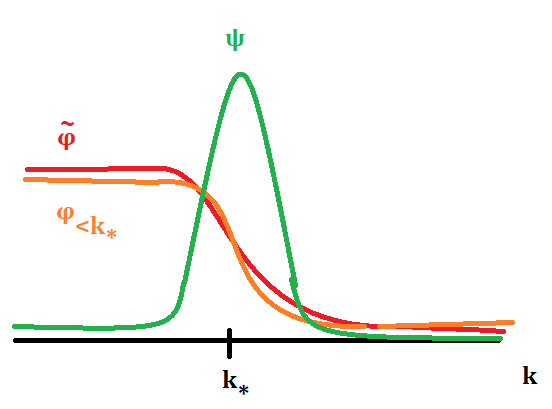
\includegraphics{graphics/envelope}
		\caption{Frequency envelopes of $\widetilde \phi$ and $\psi$. Both $\widetilde \phi$ and $P_{\leq k_*} \phi$ have the bulk of their norms below $|\xi| \sim 2^{k_*}$, and decay exponentially above, while $\psi$ decays exponentially in both directions. }
	\end{center}
\end{figure}

Using our bootstrap assumption, Moser estimates and product bounds, we can prove the following estimates 
	\begin{align}
		|| \phi_{>k_* + 10}||_{\sfS_c[J]} 
			&\lesssim 1, \\
		||(\bfS' (\widetilde\phi)\psi)_k||_{\sfS [I]}
			&\lesssim_{\widetilde \cF} c_k.
	\end{align}
	To estimate $\bfR_{1;k}$, we freely apply the $\sfS \times \sfN \to \sfN$ bound and bilinear null form estimate to write
		\begin{align*}
			||\bfR_{1;k} (\widetilde\phi, \psi)||_{\sfN[J]}
				&\lesssim ||\widetilde \phi_{< k - m}||_{\sfS[J]} \sum_{j < k - m} ||\psi_j ||_{\sfS[J]} ||\widetilde \phi_k||_{\sfS[J]}.
		\end{align*}	
	In the range $k < k_* + 10$, note that $k - m < k_*$, hence $\widetilde \psi$ is favourable, the rest can be discarded,
		\begin{align*}
			||\bfR_{1;k} (\widetilde\phi, \psi)||_{\sfN[J]} \lesssim_{\widetilde \cF} \sum_{j < k - m} c_j \lesssim_{\widetilde \cF} c_{k - m} \lesssim_{\widetilde \cF} 2^{-\delta_0 m} c_k. 
		\end{align*}
	In the range $k \geq k_* + 10$, the $\widetilde \psi_j$ term is no longer always favourable, however we gain some decay from the high frequency improvements of $\widetilde\phi_k$. 
\end{proof}




\subsubsection{High frequencies}

We now turn towards comparing the solution with truncated data $\widetilde \phi$ with the original solution $\phi$ to improve the space-time control \eqref{BS1} to \eqref{BS1i}. We claim that there exists a non-decreasing function $K_2 (\cF) > 0$ of polynomial growth such that 
	\[
		||\widetilde \phi - \phi||_{\sfS[J]} \leq K_2 (\cF). 
	\]
In view of the previous section, in which we showed that $\widetilde \phi - P_{\leq k_*} \phi$ is negligible, one can view this as an estimate on the evolution of the high frequencies of $\phi$. Given this estimate, choosing $\cF \gg \widetilde \cF \gg 1$ such that $K_2 (\widetilde \cF) \ll \cF$, it follows from the triangle inequality that
	\[
		||\phi ||_{\sfS[J]} 
			\leq ||\widetilde \phi||_{\sfS[J]} + ||\phi - \widetilde \phi||_{\sfS[J]} \leq \widetilde \cF + K_2 (\widetilde \cF) \ll \cF,
	\]
improving our space-time control \eqref{BS1} to \eqref{BS1i}, completing the bootstrap argument. 


The difference $\psi := \widetilde\phi -  \phi$ satisfies the equation
	\[
		\Box \psi
			= - \bfS (\widetilde \phi) \partial^\alpha \widetilde \phi \partial_\alpha \widetilde \phi + \bfS (\widetilde \phi + \psi) \partial^\alpha( \widetilde \phi + \psi) \partial_\alpha (\widetilde \phi + \psi).
	\]
As in the previous section, our strategy will be to reduce the problem to a perturbation of the gauge covariant equation	\eqref{linwave}. We want to apply the paradifferential argument as in the preceding proof for low frequencies, however the coefficients for this equation $\widetilde \phi$ are not small. To remedy this lack of smallness, we need three intermediate steps as outlined in the following diagram:

\begin{figure}[h]
	\begin{center}
		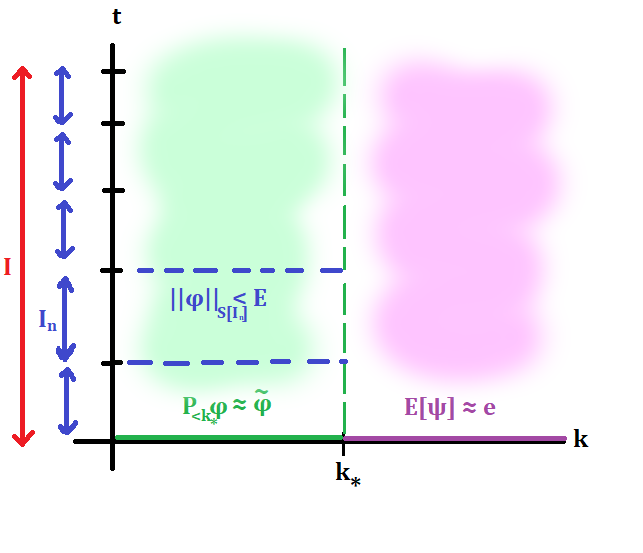
\includegraphics[scale = 0.7]{graphics/induction}
		\caption{Proposition \ref{prop:lowfreq} shows that the low frequencies are close. The high frequencies are controlled by the energy step via conservation of energy. The size of $\widetilde \phi$ in the $\sfS$-norm is large, so we divide into $O_{\widetilde \cF} (1)$-many sub-intervals on which the norm is comparable to the energy. We conclude the argument using perturbation theory on each sub-interval. 
		}
	\end{center}
\end{figure}

We first establish uniform energy bounds for $\psi$. As $\phi$ and $\widetilde\phi$ are wave maps, they have conserved energy $\cE[\phi] = \cE$ and $\cE[\widetilde \phi] \equiv \cE + e$ respectively. Thus, using Proposition \ref{prop:lowfreq}, one can conclude their difference has energy on the order $\cE[\psi] \lesssim e$. 

\begin{lemma}[Almost energy conservation]
	Let $\phi$ be a wave map with energy $\cE[\phi] = \cE + e$, and denote $\widetilde \phi$ the wave map with initial data $\widetilde \phi[0] = \Pi P_{\leq k_*} \phi[0]$ and energy $\cE[\widetilde \phi] = \cE$. If $\phi$ and $\widetilde \phi$ are defined on the time interval $J$, their difference $\psi := \phi - \widetilde \phi$ satisfies the almost conservation of energy
		\begin{equation}
			\cE[\psi(t)] \lesssim e\label{eq:psiconserve}
		\end{equation}
	for all $t \in J$. 
\end{lemma}

\begin{proof}
	Decomposing into high and low frequencies $\phi = P_{> k_*} \phi + P_{\leq k_*} \phi$ and viewing the energy as arising from the inner product on $\dot H^1 \times L^2$, we can write
		\[
			\cE[\phi] = \cE[P_{> k_*} \phi] + \cE[P_{\leq k_*} \phi] + 2 \langle P_{> k_*} \phi, P_{\leq k_*} \phi \rangle_{\dot H^1 \times L^2}.
		\]
	The Littlewood-Paley projections are non-negative operators, so the inner product on the right is non-negative. On the other hand, the estimate \eqref{lowfreq} from Proposition \ref{prop:lowfreq} states that the low frequency terms $\widetilde \phi$ and $P_{\leq k_*} \phi$ are close, so, in particular, the reverse triangle inequality implies
		\[
			\left|\cE[P_{\leq k_*} \phi] - \cE[\widetilde \phi]\right| + \left|\cE[\psi] - \cE[P_{> k_*} \phi]\right| \leq 100K_1 (\cF) \epsilon^{\delta_0}. 
		\]
	Collecting our results, we obtain
		\begin{align*}
			\cE[\psi]
				&\leq \cE[P_{> k_*} \phi] + 100 \epsilon^{\delta_0} K(\cF) \\
				&\leq \cE[\phi] - \cE[P_{\leq k_*} \phi] + 100\epsilon^{\delta_0} K(\cF)\\
				&\leq \cE[\phi] - \cE[\widetilde \phi] + 200 \epsilon^{\delta_0} K (\cF) \\
				&\leq e +  200 \epsilon^{\delta_0} K (\cF)
		\end{align*}	
	Making appropriate choices of $\epsilon$ and $\cF$ completes the proof. 	
\end{proof}

Next, we prove partial divisibility for the $\sfS$-norm. For functions with finite $L^p_t$-norm for $1 \leq p < \infty$, we can divide the interval into sub-intervals on which the $L^p_t$-norms are small. However, since the $\sfS$-norm contains $L^\infty_t$-norms, one cannot hope for divisibility into arbitrarily small norms, but one can divide into norms on the order of the energy. 


\begin{lemma}[Partial divisibility]
	Let $\widetilde \phi$ be a wave map on the interval $J$ with energy $\cE[\widetilde \phi] = \cE$ and space-time control $||\phi||_{\sfS[J]} = \widetilde \cF$. Then there exists a non-decreasing positive function $K_2 (\widetilde \cF) > 0$ of polynomial growth such that we can partition the time interval into $K_2 (\widetilde \cF)$-many sub-intervals $J = \bigsqcup J_k$ such that 
		\begin{equation}
			||\widetilde \phi||_{\sfS[J_k]} \lesssim \cE.\label{eq:divis}
		\end{equation}
\end{lemma}

\begin{proof}
	See \cite[Section 10.2]{SterbenzTataru2010}
\end{proof}

Finally, we can use the perturbation theory as in the previous section to obtain good estimates for the $\sfS$-norm of $\psi$ on each sub-interval. The coefficients $\widetilde \phi$ have size on the order of the energy, we can choose the energy step $e \ll 1$ sufficiently small, depending \textit{only} on energy, to close the continuity argument. 

\begin{proposition}[High frequency evolution]]\label{prop:highfreq}
	Let $\phi$ be a wave map with energy $\cE[\phi] = \cE + e$, and denote $\widetilde \phi$ the wave map with initial data $\widetilde \phi[0] = \Pi P_{\leq k_*} \phi[0]$ and energy $\cE[\widetilde \phi] = \cE$. If $\phi$ and $\widetilde \phi$ are defined on the time interval $J$ with bounds
		\begin{align}
			||\phi||_{\sfED[J]} 
				&\leq \epsilon, \\
			||\phi||_{\sfS[J]}
				&\leq \cF, 	
		\end{align}
	and
		\begin{align}
			||\widetilde\phi||_{\sfED[J]} 
				&\leq \widetilde\epsilon, \\
			||\widetilde\phi||_{\sfS[J]}
				&\leq \widetilde\cF, 	
		\end{align}	
	for appropriate choices of $\epsilon, \widetilde\epsilon, \cF, \widetilde\cF$, then there exists a function of energy $e(\cE)$ and a non-decreasing positive function $K_2 (\widetilde \cF) > 0$ of polynomial growth such that if $e \leq e(\cE)$ then
		\begin{equation}
			||\phi - \widetilde \phi||_{\sfS[J]} \leq K_2 (\widetilde \cF). 
		\end{equation}
\end{proposition}


\begin{proof}
	By the previous two lemmas, it suffices to consider the case where one has space-time control of $\widetilde \phi$ by the energy \eqref{divis} and prove an estimate of the form 
	\begin{equation}
		||\psi||_{\sfS[J]} \leq 1 \label{eq:pert}
	\end{equation}
	for $\psi := \phi - \widetilde \phi$. Indeed, by partitioning our overall interval, it follows from the triangle inequality that
		\[  
			||\psi||_{\sfS[J]} \leq \sum_{k = 1}^{K_2 (\widetilde \cF)} ||\psi||_{\sfS[J_k]} \leq K_2 (\widetilde \cF),
		\]
	as desired. Using the estimate \eqref{psiconserve} for $e (\cE) \ll 1$ and the energy estimate, there exists a small time interval $J_0 \subseteq J$ on which the conclusion \eqref{pert} holds. We propagate this base case by making the bootstrap assumption
		\begin{equation}
			||\psi||_{\sfS[I]} \leq 2
		\label{eq:pertBA}
		\end{equation}
	for some sub-interval $I \subseteq J$, and aim to improve to \eqref{pert}. The difference satisfies the equation
	\begin{equation}
		\Box \psi
			= - \bfS (\widetilde \phi) \partial^\alpha \widetilde \phi \partial_\alpha \widetilde \phi + \bfS (\widetilde \phi + \psi) \partial^\alpha( \widetilde \phi + \psi) \partial_\alpha (\widetilde \phi + \psi).
	\end{equation}
	To close the bootstrap argument, we project to each frequency $|\xi| \sim 2^k$, obtaining the linear paradifferential form for the equation, and apply the gauge covariant estimate \eqref{renormest}
		\begin{equation}
			\Box \psi_k + 2 \bfA^\alpha (\phi)_{< k - m} \partial_\alpha \psi_k = \frT^m_k (\widetilde \phi) + \frT^m_k (\widetilde \phi + \psi) + \frL^m_k (\widetilde \phi, \psi)
		\end{equation}
	where $\frT^m_k$ denotes a matched frequency trilinear expression, and $\frL^m_k$ contains the low-high-low and low-low-high interactions, 
		\begin{align*}
			\frL_k^m  (\widetilde \phi, \psi)
				&= - \left( \bfA^\alpha (\widetilde \phi + \psi)_{<k - m} - \bfA^\alpha (\widetilde \phi)_{< k - m} \right) \partial_\alpha \widetilde \phi_k \\
				&= -\bfS(\widetilde\phi)_{< k - m} \partial^\alpha \psi_{<k - m} \partial_\alpha \widetilde \phi_k + \left( \bfS' (\widetilde\phi) \psi \right)_{< k - m} \partial^\alpha \widetilde\phi_{<k - m} \partial_\alpha \widetilde\phi_k = \bfR_{1;k}  (\widetilde \phi, \psi)+ \bfR_{2;k} (\widetilde \phi, \psi).
		\end{align*}
	Here we have abused notation to write $\bfS$ for the anti-symmetrisation of the second fundamental form. It remains to show that the right-hand side of our paradifferential equation is indeed perturbative. The matched frequencies $\frT_k^m$ can be dealt with easily by the energy dispersion estimates, while the separated frequency interactions in $\frL_k^m$ need to be treated more carefully. The latter will be our focus. In view of the low frequency results from Proposition \ref{prop:lowfreq}, we can restrict our attention to high frequencies $k \geq k_* - 10$. 
	\begin{figure}[h]
	\begin{center}
		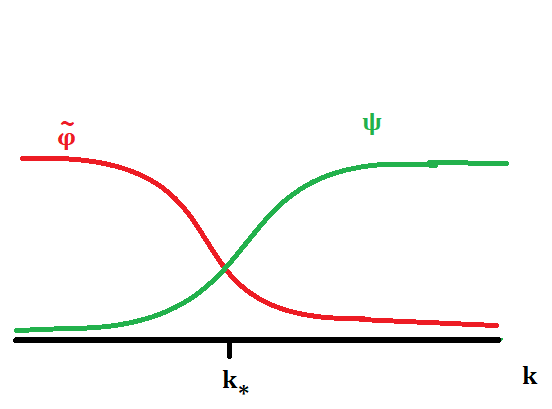
\includegraphics{graphics/envelope2}
		\caption{Frequency envelopes of $\widetilde \phi$ and $\psi$. The former has the bulk of its norm below $|\xi| \sim 2^{k_*}$ and decays exponentially above, while the latter has the bulk of its norm above and decays exponentially below. }
	\end{center}
\end{figure}

	Using the frequency envelope refinements for the low frequency evolution estimates and Moser estimates for the second fundamental form, we have the following estimates
		\begin{align}
			||\widetilde \phi_k||_{\sfS[J]}
				&\lesssim 2^{-\delta_0 (k - k_*)_+},\\
			||\psi_k||_{\sfS[J]}
				&\lesssim 2^{-\delta_0 (k_* - k)_+},\\	
			||(\bfS' (\widetilde \phi)\psi)_k||_{\sfS[J]}
				&\lesssim 2^{-\delta_0 (k_* - k)_+},\\
			||\bfS' (\widetilde \phi)\psi||_{\sfS[J]}
				&\lesssim 1.		
		\end{align}	
	To estimate $\bfR_{1;k}$, we freely apply the $\sfS \times \sfN \to \sfN$ bound and bilinear null form estimate to write 
		\begin{align*}
			||\bfR_{1;k}(\widetilde\phi, \psi)||_{\sfN[J]}
				&\lesssim ||\widetilde \phi_{< k - m}||_{\sfS[J]} \sum_{j < k - m} ||\psi_j||_{\sfS[J]} ||\widetilde\phi_k||_{\sfS[J]}\\
				&\lesssim_\cE \sum_{j < k - m} 2^{-\delta (k_* - j)_+} 2^{-\delta( k - k_*)_+}.
		\end{align*}	
	When $k_* - 10 \leq k \leq k_* + m$, the right-hand side is controlled by $2^{-\delta m}$. When $k > k_* + m$, the right-hand side is controlled by $|k - k_*| 2^{-\delta (k - k_*)}$. We conclude
		\[
			||\bfR_{1;k}(\widetilde\phi, \psi)||_{\sfN[J]}
				\lesssim 2^{-\frac14 \delta m} 2^{-\frac12\delta (k - k_*)}.
		\]
	The first factor on the right guarantees smallness, the second factor on the right guarantees summability. The estimate for $\bfR_{2;k}$ is similar. 
\end{proof}